% This is samplepaper.tex, a sample chapter demonstrating the
% LLNCS macro package for Springer Computer Science proceedings;
% Version 2.20 of 2017/10/04
%
\documentclass[runningheads]{llncs}
%
%\usepackage[T2A]{fontenc}
%\usepackage[utf8]{inputenc}
%\usepackage[english,russian]{babel}
\usepackage[linesnumberedhidden,lined,ruled]{algorithm2e}

\usepackage[colorlinks=true,urlcolor=blue,linkcolor=blue,citecolor=blue]{hyperref}
\usepackage{amsmath}
\usepackage{amssymb}
\usepackage{doi}
\usepackage{tikz,tikz-3dplot}
\usetikzlibrary{graphs}
\usetikzlibrary{graphs.standard}
\newcommand{\R}{\mathbb{R}}  
\newcommand{\Z}{\mathbb{Z}}  
\newcommand{\N}{\mathbb{N}} 
\DeclareMathOperator\conv {conv} 
\DeclareMathOperator\TSP {TSP} 
\DeclareMathOperator\ATSP {ATSP}
%\newtheorem {Theorem} {Theorem}
%\newtheorem {Lemma} [Theorem] {Lemma}
\setlength{\belowcaptionskip}{-1ex}

\usepackage{graphicx}
% Used for displaying a sample figure. If possible, figure files should
% be included in EPS format.
%
% If you use the hyperref package, please uncomment the following line
% to display URLs in blue roman font according to Springer's eBook style:
% \renewcommand\UrlFont{\color{blue}\rmfamily}

\begin{document}
%
\title{Simulated annealing approach to verify vertex adjacencies in the traveling salesperson polytope}
%
\titlerunning{SA approach to verify vertex adjacencies in the TSP polytope}
% If the paper title is too long for the running head, you can set
% an abbreviated paper title here
%
\author{Anna Kozlova\inst{1} \and
Andrei Nikolaev\inst{1}}
%
\authorrunning{Kozlova A.\,P, Nikolaev A.\,V.}
% First names are abbreviated in the running head.
% If there are more than two authors, 'et al.' is used.
%
\institute{P.\,G. Demidov Yaroslavl State University\\
\email{fyz95@mail.ru, andrei.v.nikolaev@gmail.com}}
%
\maketitle              % typeset the header of the contribution
%
\begin{abstract}
We consider 1-skeletons of the symmetric and asymmetric traveling salesperson polytopes whose vertices are all possible Hamiltonian tours in the complete directed or undirected graph, and the edges are geometric edges or one-dimensional faces of the polytope.
It is known that the question whether two vertices of the symmetric or asymmetric traveling salesperson polytopes are nonadjacent is NP-complete.
A sufficient condition for nonadjacency can be formulated as a combinatorial problem: if from the edges of two Hamiltonian tours we can construct two complementary Hamiltonian tours, then the corresponding vertices of the traveling salesperson polytope are not adjacent. 
We consider a heuristic simulated annealing approach to solve this problem. It is based on finding a vertex-disjoint cycle cover and a perfect matching.
The algorithm has a one-sided error: the answer ``not adjacent'' is always correct, and was tested on random and pyramidal Hamiltonian tours.


\keywords{traveling salesperson problem \and Hamiltonian tour \and traveling salesperson polytope \and 1-skeleton \and vertex adjacency \and simulated annealing \and vertex-disjoint cycle cover \and perfect matching.}
\end{abstract}
%
%
%

\section{Introduction} %Введение 

We consider a classical traveling salesperson problem on a complete directed or undirected graph. 

\textsc{Symmetric traveling salesperson problem.} Given a complete weighted graph $K_n=(V,E)$, it is required to find a Hamiltonian cycle of minimum weight.

\textsc{Asymmetric traveling salesperson problem.} Given a complete weighted digraph $D_n=(V,A)$, it is required to find a Hamiltonian tour of minimum weight.

%Further, we call Hamiltonian cycles in both directed and undirected graphs as Hamiltonian tours.

We denote by $HC_n$ the set of all Hamiltonian cycles in $K_n$ and by $HT_n$ the set of all Hamiltonian tours in $D_n$. With each Hamiltonian cycle $x \in HC_n$ we associate a characteristic vector $x^v \in \R^{E}$ by the following rule:
\[
x^v_e = 
\begin{cases}
1,& \text{ if the cycle } x \text{ contains an edge } e \in E,\\
0,& \text{ otherwise. }
\end{cases}
\]
With each Hamiltonian tour $y \in HT_n$ we associate a characteristic vector $y^v \in \R^{A}$ by the following rule:
\[
y^v_a = 
\begin{cases}
1,& \text{ if the tour } y \text{ contains an edge } a \in A,\\
0,& \text{ otherwise. }
%1,& \text{ если дуга } a \in A \text{ входит в контур } y,\\
%0,& \text{ в противном случае.}
\end{cases}
\]
The polytope %Многогранник
\[\TSP(n) = \conv \{x^v \ | \ x \in HC_n \}\]
is called \textit{the symmetric traveling salesperson polytope},  %называется \textit{симметричным многогранником задачи коммивояжёра}.
and the polytope %Многогранник
\[\ATSP(n) = \conv \{y^v \ | \ y \in HT_n \}\]
is called \textit{the asymmetric traveling salesperson polytope}.%называется \textit{асимметричным многогранником задачи коммивояжёра}.

The $1$-skeleton of a polytope $P$ is the graph whose vertex set is the vertex set of $P$ (characteristic vectors $x^v$ for the traveling salesperson problem) and edge set is the set of geometric edges or one-dimensional faces of $P$. Many papers are devoted to the study of $1$-skeletons associated with combinatorial problems. On the one hand, the vertex adjacency in $1$-skeleton is of great interest for the development of algorithms to solve problems based on local search technique (when we choose the next solution as the best one among adjacent solutions). For example, various algorithms for perfect matching, set covering, independent set, ranking of objects, problems with fuzzy measures, and many others are based on this idea \cite{Aguilera,Balinski,Chegireddy,Combarro,Gabow,Matsui}. On the other hand, some characteristics of $1$-skeletons, such as the diameter and the clique number, estimate the time complexity for different computation models and classes of algorithms \cite{Bondarenko,Bondarenko-Maksimenko,Bondarenko-Nikolaev-2017,Grotschel}.
%Полиэдральным графом задачи называется граф, вершинами которого являются вершины многогранника (характеристические векторы для задачи коммивояжёра), а рёбрами --- геометрические рёбра, т.е. одномерные грани. Исследованию полиэдральных графов труднорешаемых задач посвящено значительное число работ. С одной стороны, смежность вершин в полиэдральном графе представляет наибольший интерес для непосредственной разработки алгоритмов решения задач, основанных на методах локального поиска (когда от текущего решения переход осуществляется к «лучшему» решению среди смежных). На этой идее основаны, например, различные алгоритмы для задачи о совершенном паросочетании, покрытии множества, независимом множестве, ранжировании объектов, задачи с нечёткими мерами и многие другие \cite{Aguilera,Balinski,Chegireddy,Combarro,Gabow,Matsui}. С другой стороны, различные характеристики полиэдрального графа задачи, такие как диаметр и кликовое число, служат оценками сложности для различных моделей вычислений и классов алгоритмов \cite{Bondarenko,Bondarenko-Maksimenko,Bondarenko-Nikolaev-2017,Grotschel}.

Unfortunately, the classical result by Papadimitriou states that the construction of 1-skeleton of the traveling salesperson polytope is NP-complete for both directed and undirected graphs.
%К сожалению, классический результат Пападимитриу говорит о том, что задача построения полиэдрального графа задачи коммивояжёра является сложной как для ориентированных, так и для неориентированных графов.
\begin{theorem} [Papadimitriou, \cite{Papadimitriou}]
    The question whether two vertices of the polytopes $\TSP(n)$ or $\ATSP(n)$ are nonadjacent is NP-complete. 
	%Задача проверки несмежности вершин в многогранниках $\TSP(n)$ и $\ATSP(n)$ является NP"~полной.	
\end{theorem}

However, the vertex adjacency test for $\TSP(n)$ and $\ATSP(n)$ is an interesting problem itself. Note that a geometric approach to the construction of 1-skeleton of the traveling salesperson polytope seems not very promising because both polytopes have superexponential number of vertices and faces \cite{Fiorini,Grotschel}.
%Тем не менее, проверка смежности вершин многогранников $\TSP(n)$ и $\ATSP(n)$ представляет собой интересную практическую задачу. Отметим, что геометрический подход к построению полиэдрального графа задачи коммивояжёра представляется малоперспективным, так как оба многогранника обладают сверхэкспоненциальным числом вершин и гиперграней \cite{Fiorini,Grotschel}.

In \cite{Rao} the sufficient condition for vertex adjacency in the traveling salesperson polytope was reformulated in a combinatorial form.
%В работе \cite{Rao} условия смежности вершин многогранников задачи коммивояжёра были переформулированы в комбинаторном виде.

\begin{lemma}[Sufficient condition for nonadjacency] \label{lemma_nonadjacency}
	If from the edges of \break
	two Hamiltonian tours $x$ and $y$ it is possible to construct two complementary Hamiltonian tours $z$ and $w$, then the corresponding vertices $x^v$ and $y^v$ of the polytope $\TSP(n)$ (or $\ATSP(n)$) are not adjacent. %Если из рёбер гамильтоновых циклов (контуров) $x$ и $y$ можно составить два дополнительных гамильтоновых цикла (контура) $z$ и $w$, то вершины $x^v$ и $y^v$ многогранника $\TSP(n)$ (многогранника $\ATSP(n)$) не смежны.
\end{lemma}

From the geometric point of view, the Lemma~\ref{lemma_nonadjacency} means that the segment connecting two vertices $x^v$ and $y^v$ intersects with the segment connecting two other vertices $z^v$ and $w^v$ of the polytope $\TSP(n)$ (or $\ATSP(n)$ correspondingly), thus it cannot be an edge in 1-skeleton. An example of a satisfied sufficient condition is shown in Fig.~\ref{image1}. % С геометрической точки зрения условие из леммы~\ref{lemma_nonadjacency} означает, что отрезок, соединяющий вершины $x^v$ и $y^v$, пересекается с отрезком, соединяющим две других вершины $z^v$ и $w^v$ многогранника $\TSP(n)$ ($\ATSP(n)$ соответственно), а значит не может являться ребром многогранника. Пример выполнения достаточного условия приведён на \autoref{image1}. 

\begin{figure}[t]
	\centering
	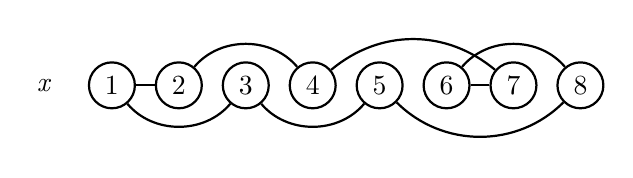
\begin{tikzpicture}[scale=0.85]
	\begin{scope}[every node/.style={circle,thick,draw,inner sep=3pt}]
	\node (A) at (0,0) {1};
	\node (B) at (1,0) {2};
	\node (C) at (2,0) {3};
	\node (D) at (3,0) {4};
	\node (E) at (4,0) {5};
	\node (F) at (5,0) {6};
	\node (G) at (6,0) {7};
	\node (H) at (7,0) {8};
	\end{scope}
	\draw [thick] (A) edge (B);
	\draw [thick] (B) edge [bend left=50] (D);
	\draw [thick] (D) edge [bend left=40] (G);
	\draw [thick] (G) edge (F);
	\draw [thick] (F) edge [bend left=50] (H);
	\draw [thick] (H) edge [bend left=45] (E);
	\draw [thick] (E) edge [bend left=50] (C);
	\draw [thick] (C) edge [bend left=50] (A);
	\draw (-1, 0) node{\textit{x}};
	\end{tikzpicture}
	\\
	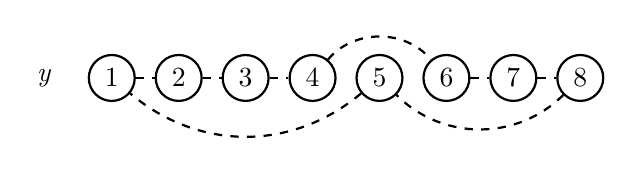
\begin{tikzpicture}[scale=0.85]
	\begin{scope}[every node/.style={circle,thick,draw,inner sep=3pt}]
	\node (A) at (0,0) {1};
	\node (B) at (1,0) {2};
	\node (C) at (2,0) {3};
	\node (D) at (3,0) {4};
	\node (E) at (4,0) {5};
	\node (F) at (5,0) {6};
	\node (G) at (6,0) {7};
	\node (H) at (7,0) {8};
	\end{scope}
	\draw [thick,dashed] (A) edge (B);
	\draw [thick,dashed] (B) edge (C);
	\draw [thick,dashed] (C) edge (D);
	\draw [thick,dashed] (D) edge [bend left=50] (F);
	\draw [thick,dashed] (F) edge (G);
	\draw [thick,dashed] (G) edge (H);
	\draw [thick,dashed] (H) edge [bend left=45] (E);
	\draw [thick,dashed] (E) edge [bend left=40] (A);
	\draw (-1, 0) node{\textit{y}};
	\end{tikzpicture}
	\\
	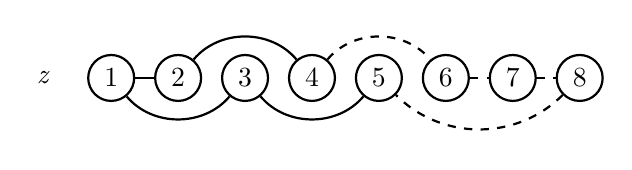
\begin{tikzpicture}[scale=0.85]
	\begin{scope}[every node/.style={circle,thick,draw,inner sep=3pt}]
	\node (A) at (0,0) {1};
	\node (B) at (1,0) {2};
	\node (C) at (2,0) {3};
	\node (D) at (3,0) {4};
	\node (E) at (4,0) {5};
	\node (F) at (5,0) {6};
	\node (G) at (6,0) {7};
	\node (H) at (7,0) {8};
	\end{scope}
	\draw [thick] (A) edge (B);
	\draw [thick] (B) edge [bend left=50] (D);
	\draw [thick,dashed] (D) edge [bend left=50] (F);
	\draw [thick,dashed] (F) edge (G);
	\draw [thick,dashed] (G) edge (H);
	\draw [thick,dashed] (H) edge [bend left=45] (E);
	\draw [thick] (E) edge [bend left=50] (C);
	\draw [thick] (C) edge [bend left=50] (A);
	\draw (-1, 0) node{\textit{z}};
	\end{tikzpicture}
	\\
	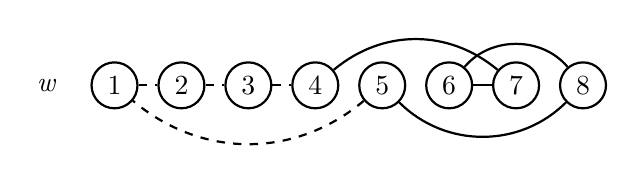
\begin{tikzpicture}[scale=0.85]
	\begin{scope}[every node/.style={circle,thick,draw,inner sep=3pt}]
	\node (A) at (0,0) {1};
	\node (B) at (1,0) {2};
	\node (C) at (2,0) {3};
	\node (D) at (3,0) {4};
	\node (E) at (4,0) {5};
	\node (F) at (5,0) {6};
	\node (G) at (6,0) {7};
	\node (H) at (7,0) {8};
	\end{scope}
	\draw [thick,dashed] (A) edge (B);
	\draw [thick,dashed] (B) edge (C);
	\draw [thick,dashed] (C) edge (D);
	\draw [thick] (D) edge [bend left=40] (G);
	\draw [thick] (G) edge (F);
	\draw [thick] (F) edge [bend left=50] (H);
	\draw [thick] (H) edge [bend left=45] (E);
	\draw [thick,dashed] (E) edge [bend left=40] (A);
	\draw (-1, 0) node{\textit{w}};
	\end{tikzpicture}
	\caption{Two complementary tours $z$ and $w$ are constructed from the edges of $x$ and $y$}
	%\caption{Пример двух дополнительных циклов $z$ и $w$, полученных из рёбер $x$ и $y$}
	\label{image1}
\end{figure}

Let us formulate the sufficient condition for vertex nonadjacency of the traveling salesperson polytope in the form of a combinatorial problem. \\ %Сформулируем достаточное условие несмежности вершин многогранника коммивояжёра в виде комбинаторной задачи.\\
\textsc{Instance.} Let $x$ and $y$ be two Hamiltonian tours.\\ %\textsc{Условие.} Заданы два гамильтоновых цикла (контура) $x$ и $y$.\\
\textsc{Question.} Does the multigraph $x \cup y$ include a pair of Hamiltonian tours $z$ and $w$ different from $x$ and $y$ such that %\textsc{Вопрос.} Найдутся ли в мультиграфе $x \cup y$ два гамильтоновых цикла (контура) $z$ и $w$, отличных от $x$ и $y$, что
\[z \cup w = x \cup y \text{ and } z \cap w = \emptyset?\]

By $x \cup y$ we denote a multigraph that contains all edges of both tours $x$ and $y$ (Fig.~\ref{image2}).
%Через $x \cup y$ мы обозначаем мультиграф, который содержит все рёбра циклов $x$ и $y$.

In this formulation, the problem is close to the $2$-peripatetic salesperson problem in which it is required to find two Hamiltonian tours of minimum weight without common edges. The $2$-peripatetic salesperson is NP-complete even for $4$-regular graphs \cite{DeKort}. Much attention was paid to the development of approximation algorithms for this problem (see, for example, \cite{Ageev,Baburin,Glebov}). %В такой формулировке задача близка к задаче о двух коммивояжёрах (2-peripatetic salesman problem), которая заключается в поиске в графе двух гамильтоновых циклов минимального веса, не имеющих общих рёбер. Задача о двух коммивояжёрах является NP-полной уже для 4-регулярных графов \cite{DeKort}. Значительное число работ посвящено построению для неё приближённых алгоритмов (см., например, \cite{Ageev,Baburin,Glebov}).

However, the combinatorial form of the sufficient condition for nonadjacency has a number of differences from the $2$-peripatetic salesperson problem: %Однако, задача в достаточном условии несмежности вершин имеет ряд отличий от задачи о двух коммивояжёрах: 
\begin{itemize}
	\item this is a decision problem, not an optimization one; %рассматриваемая задача является задачей распознавания, а не оптимизации;
	\item the graph is a $4$-regular graph (or digraph) of a special form constructed as a union of two Hamiltonian tours; % граф в задаче представляет собой 4-регулярный граф (орграф) специального вида, построенный как объединение двух гамильтоновых циклов (контуров);
	\item it is required to find two Hamiltonian tours different from $x$ and $y$. % по условию задачи в мультиграфе $x \cup y$ требуется найти два гамильтоновых цикла (контура), отличных от заданных циклов $x$ и $y$. 
\end{itemize}

Note also that if from the edges of two Hamiltonian tours $x$ and $y$ it is possible to construct another Hamiltonian tour $z$, then all the remaining edges $(x \cup y) \backslash z$ are almost certainly do not form a Hamiltonian tour (Fig.~\ref{image2}). Thus, instead of algorithms for a single Hamiltonian tour in the multigraph $x \cup y$, in this paper we consider a heuristic simulated annealing approach to test vertex adjacencies in the symmetric and asymmetric traveling salesperson polytopes based on finding a vertex-disjoint cycle cover and a perfect matching. % Отметим также, что если из рёбер гамильтоновых циклов $x$ и $y$ можно собрать отличный от них гамильтонов цикл $z$, то все оставшиеся рёбра $(x \cup y) \backslash z$ с высокой вероятностью не образуют гамильтонова цикла (\autoref{image2}). Поэтому вместо алгоритмов поиска гамильтоновых циклов в мультиграфе $x \cup y$, в данной работе рассматривается эвристический алгоритм имитации отжига проверки несмежности вершин симметричного и асимметричного многогранников коммивояжёра, основанный на покрытии графа циклами и построении совершенных паросочетаний.

\begin{figure}[t]
	\centering
	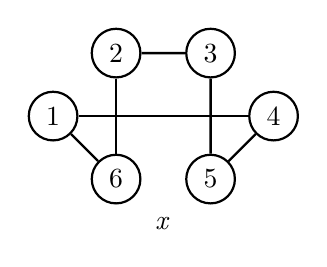
\begin{tikzpicture}[scale=0.8]
	\begin{scope}[every node/.style={circle,thick,draw}]
	\node (A) at (0,0) {1};
	\node (B) at (1,1) {2};
	\node (C) at (2.5,1) {3};
	\node (D) at (3.5,0) {4};
	\node (E) at (2.5,-1) {5};
	\node (F) at (1,-1) {6};
	\end{scope}
	\draw [line width=0.3mm] (A) edge (D);
	\draw [line width=0.3mm] (D) edge (E);
	\draw [line width=0.3mm] (E) edge (C);
	\draw [line width=0.3mm] (C) edge (B);
	\draw [line width=0.3mm] (B) edge (F);
	\draw [line width=0.3mm] (F) edge (A);
	\draw (1.75, -1.7) node{\textit{x}};
	\end{tikzpicture}
	\hspace*{6mm}
	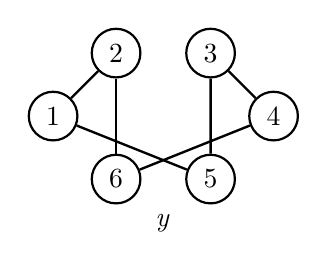
\begin{tikzpicture}[scale=0.8]
	\begin{scope}[every node/.style={circle,thick,draw}]
	\node (A) at (0,0) {1};
	\node (B) at (1,1) {2};
	\node (C) at (2.5,1) {3};
	\node (D) at (3.5,0) {4};
	\node (E) at (2.5,-1) {5};
	\node (F) at (1,-1) {6};
	\end{scope}
	\draw [line width=0.3mm] (A) edge (B);
	\draw [line width=0.3mm] (B) edge (F);
	\draw [line width=0.3mm] (F) edge (D);
	\draw [line width=0.3mm] (D) edge (C);
	\draw [line width=0.3mm] (C) edge (E);
	\draw [line width=0.3mm] (E) edge (A);
	\draw (1.75, -1.7) node{\textit{y}};
	\end{tikzpicture}
	\\
	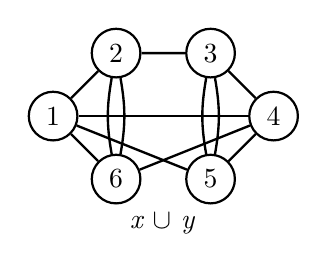
\begin{tikzpicture}[scale=0.8]
	\begin{scope}[every node/.style={circle,thick,draw}]
	\node (A) at (0,0) {1};
	\node (B) at (1,1) {2};
	\node (C) at (2.5,1) {3};
	\node (D) at (3.5,0) {4};
	\node (E) at (2.5,-1) {5};
	\node (F) at (1,-1) {6};
	\end{scope}
	\draw [line width=0.3mm] (A) edge (D);
	\draw [line width=0.3mm] (D) edge (E);
	\draw [line width=0.3mm, bend right=10] (E) edge (C);
	\draw [line width=0.3mm] (C) edge (B);
	\draw [line width=0.3mm, bend right=10] (B) edge (F);
	\draw [line width=0.3mm] (F) edge (A);
	\draw [line width=0.3mm] (A) edge (B);
	\draw [line width=0.3mm, bend left=10] (B) edge (F);
	\draw [line width=0.3mm] (F) edge (D);
	\draw [line width=0.3mm] (D) edge (C);
	\draw [line width=0.3mm, bend right=10] (C) edge (E);
	\draw [line width=0.3mm] (E) edge (A);
	\draw (1.75, -1.7) node{\textit{x $\cup$ y}};
	\end{tikzpicture}
	\\
	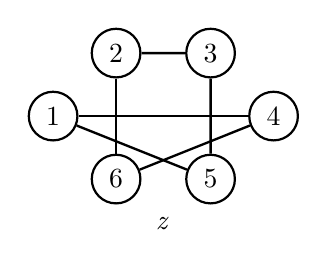
\begin{tikzpicture}[scale=0.8]
	\begin{scope}[every node/.style={circle,thick,draw}]
	\node (A) at (0,0) {1};
	\node (B) at (1,1) {2};
	\node (C) at (2.5,1) {3};
	\node (D) at (3.5,0) {4};
	\node (E) at (2.5,-1) {5};
	\node (F) at (1,-1) {6};
	\end{scope}
	\draw [line width=0.3mm] (A) edge (D);
	\draw [line width=0.3mm] (D) edge (F);
	\draw [line width=0.3mm] (F) edge (B);
	\draw [line width=0.3mm] (B) edge (C);
	\draw [line width=0.3mm] (C) edge (E);
	\draw [line width=0.3mm] (E) edge (A);
	\draw (1.75, -1.7) node{\textit{z}};
	\end{tikzpicture}
	\hspace*{6mm}
	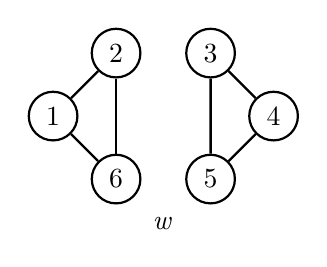
\begin{tikzpicture}[scale=0.8]
	\begin{scope}[every node/.style={circle,thick,draw}]
	\node (A) at (0,0) {1};
	\node (B) at (1,1) {2};
	\node (C) at (2.5,1) {3};
	\node (D) at (3.5,0) {4};
	\node (E) at (2.5,-1) {5};
	\node (F) at (1,-1) {6};
	\end{scope}
	\draw [line width=0.3mm] (A) edge (B);
	\draw [line width=0.3mm] (B) edge (F);
	\draw [line width=0.3mm] (F) edge (A);
	\draw [line width=0.3mm] (C) edge (D);
	\draw [line width=0.3mm] (D) edge (E);
	\draw [line width=0.3mm] (E) edge (C);
	\draw (1.75, -1.7) node{\textit{w}};
	\end{tikzpicture}
	%\caption{Пример $w = (z \cup y) \backslash z$, не являющегося гамильтоновым циклом}
	\caption{An example of $w = (z \cup y) \backslash z$ that is not a Hamiltonian tour}
	\label{image2}
\end{figure}

\section{Simulated annealing} % \section{Общая схема алгоритма имитации отжига} 
The simulated annealing borrows the concept from annealing in metallurgy where a metal material is repeatedly heated, kneaded, and cooled to enlarge the size of its crystals to
eliminate defects~\cite{Kirkpatrick}.

We consider a general scheme of the Algorithm~\ref{simmanneal}.
It is required to minimize the energy function specified for the current system state. The algorithm starts from a certain initial state: at each step a neighbor candidate state is generated which energy is compared to the energy of the previous state. If the energy decreases, the system transits to the new state, otherwise it may transit with a certain probability (to prevent falling into the local minimum). %Требуется минимизировать функцию энергии, заданную для текущего состояния системы. Алгоритм начинает работу с некоторого начального состояния: генерируется состояние"=кандидат, для которого вычисляется энергия и сравнивается с энергией предыдущего состояния. Если энергия уменьшилась, то переход в новое состояние осуществляется однозначно, иначе переход осущетсвляется с некоторой вероятностью (для предотвращения застревания в локальном минимуме функции энергии).

The algorithm receives input data in one of the following formats: %На вход алгоритму подаются данные в одном из форматов:
\begin{enumerate}
    \item Two Hamiltonian tours $x = [a_1, \ldots, a_N]$ and $y = [b_1, \ldots, b_N]$, given as the permutations of vertices in a complete graph (or digraph) $K_N$; % $2$ гамильтоновых цикла (контура) $x = [a_1, \ldots, a_N]$ и $y = [b_1, \ldots, b_N]$ в~полном графе $K_N$, в виде перестановки всех его вершин
    \item $2/4$-regular graph ($2$~--- for directed and $4$~--- for undirected graphs) of size $N$, i.e. the union of two Hamiltonian tours, given as the adjacency list. %\item $2/4$"~регулярный граф ($2$~--- для ориентированных и $4$~--- для неориентированных графов) размерности $N$, т.е. объединение $2$ циклов; задаётся в виде списка смежности.
\end{enumerate}

Other input parameters: the initial value of temperature $initT$, the maximum number of iterations $iterN$, and the the size of a queue of fixed edges $fixEdgesN$.
The algorithm stops when the solution is found or when the number of iterations exceeds the value of the parameter $iterN$.
%Помимо этого, на вход подаются параметры $\texttt{-{}-}t_{\max}$ и $\texttt{-{}-}t_{\min}$~--- максимальная и минимальная температура, которая на каждом шаге будет уменьшаться. Алгоритм прекратит работу, достигнув минимальной температуры, либо когда пройдет все допустимые итерации, заданные параметром $\texttt{-{}-}iterN$.
As an output, the algorithms returns two complementary Hamiltonian tours $z$ and $w$ constructed from the edges of $x$ and $y$. By the sufficient condition (Lemma~\ref{lemma_nonadjacency}), the corresponding vertices $x^v$ and $y^v$ of the traveling salesperson polytope are not adjacent. %На выходе будут получены два новых гамильтоновых цикла (контура) $z$ и $w$, образованные путем перестановок рёбер в исходных графах. По достаточному условию несмежности (лемма~\ref{lemma_nonadjacency} соответствующие вершины многогранника задачи коммивояжёра гарантировано не смежны).
If the algorithm cannot find the complementary tours, then it returns that the corresponding vertices are probably adjacent. Thus, the algorithm has a one-sided error: the answer ``not adjacent'' is always correct, while the answer ``probably adjacent'' leaves the possibility that the vertices actually are not adjacent. %Если алгоритм не смог найти дополнительные циклы, то делается вывод о возможной смежности соответствующих вершин. Таким образом, алгоритм является алгоритмом с односторонней ошибкой: ответ <<не смежны>> всегда корректен, ответ <<возможно не смежны>> оставляет задачу открытой.

\SetAlgorithmName{Algorithm}{Algorithm list}{} 
\SetAlgoCaptionSeparator{.} 
\DontPrintSemicolon
\SetKwProg{Proc}{Procedure}{}{End}
\SetKw{Return}{Return}
%\SetKwFor{While}{Пока}{}{Конец}
\SetKwFor{For}{For}{}{End}
\SetKw{KwTo}{to}
\SetKw{KwOr}{or}
\SetKwIF{If}{ElseIf}{Else}{If}{Then}{Else}{Else}{End}
\begin{algorithm}[t]
    \label{simmanneal}
	\caption{Simulated Annealing Algorithm}
	\SetKwInOut{Input}{Input}
	\SetKwInOut{Output}{Output}
	\SetKwData{x}{$x$}
	\SetKwData{y}{$y$}
	\SetKwData{combinedGraph}{$combG$}
	\SetKwData{startTemp}{$initT$}
	\SetKwData{finishTemp}{$finalT$}
	\SetKwData{numOfIterations}{$iterN$}
	\SetKwData{numOfEdgesToFix}{$fixEdgesN$}
	\SetKwData{T}{$T$}
	\SetKwData{candidateEnergy}{$candE$}
	\SetKwData{zCand}{$zCand$}
	\SetKwData{wCand}{$wCand$}
	\SetKwData{currentEnergy}{$currE$}
	%\SetKwData{P}{$P$}
	\SetKwData{z}{$z$}
	\SetKwData{w}{$w$}
	\SetKwData{k}{$k$}
	\SetKwData{true}{true}
	\SetKwData{false}{false}
	\SetKwData{or}{$OR$}
	\SetKwData{and}{$AND$}
	\SetKwData{SimulatedAnnealing}{$SimulatedAnnealing$}
	\SetKwData{getInitialState}{$GetInitialState$}
	\SetKwData{calculateEnergy}{$CalculateEnergy$}
	\SetKwData{transitToNewState}{$TransitToNewState$}
	\SetKwData{generateNeighbourCandidate}{$GenerateNeighbourCandidate$}
	\SetKwFunction{shouldAcceptCandidate}{$ShouldAcceptCandidate$}
	\SetKwFunction{coolingSchedule}{$CoolingSchedule$}
	\SetKwData{TestVertexAdjacency}{$TestVertexAdjacency$}
	
	\Input{ 
	    Hamiltonian tours \x and \y (or $2$/$4$-regular graph \combinedGraph), \newline 
	    initial temperature \startTemp, %and final temperature \finishTemp, 
	    number of iterations \numOfIterations, size of a queue of fixed edges \numOfEdgesToFix
	    %циклы \x и \y (или 2/4"~регулярный граф \combinedGraph), \newline 
	    %начальная температура \startTemp и конечная температура \finishTemp, \newline
	    %число итераций \numOfIterations, \newline 
	    %число зафиксированных рёбер \numOfEdgesToFix
	}
	\Output{ vertices $x^v$ and $y^v$ are adjacent or not adjacent, complementary Hamiltonian tours \z and \w, if exist}
	\BlankLine
	\Proc{\SimulatedAnnealing{\x, \y, \combinedGraph, \startTemp, 
	%\numOfEdgesToExchage, \numOfAnswersToGenerate,
	\numOfEdgesToFix}}{
	    \T $\leftarrow$ \startTemp\;
		\z, \w $\leftarrow$ \getInitialState{\x, \y, \combinedGraph}\;
			
		\For{$k\leftarrow 1$ \KwTo \numOfIterations}{
		    %\For{$a\leftarrow 1$ \KwTo \numOfAnswersToGenerate}{
    		    \If{\z and \w are Hamiltonian tours different from \x and \y}{
    		        \Return \z and \w\;
    		    }
    		  
		        \zCand, \wCand $\leftarrow$ \generateNeighbourCandidate{\z, \w, \numOfEdgesToFix}\;
    		    \candidateEnergy $\leftarrow$ \calculateEnergy{\zCand, \wCand} \;
    		    
    		    \If{\candidateEnergy \textless \currentEnergy \KwOr \shouldAcceptCandidate{}}{
    		        \z $\leftarrow$ \zCand, \w $\leftarrow$ \wCand\;
    		    }
    		   
    		    \T $\leftarrow$ \coolingSchedule{\k}\;
    		  
    		%    \If{\T \textless \finishTemp}{
    		%        \Return no complementary tours found;
    		%    }
		    %}
		}
		\Return no complementary tours found;
  }\;
\Proc{\TestVertexAdjacency{\x, \y, \combinedGraph, \startTemp, \numOfEdgesToFix}}{
	\z, \w  $\leftarrow$ \SimulatedAnnealing{\x, \y, \combinedGraph, \startTemp, \numOfEdgesToFix}
	
	\eIf{\z and \w are not empty}{
		\Return vertices $x^v$ and $y^v$ are not adjacent\;
	}{
		\Return vertices $x^v$ and $y^v$  are probably adjacent\;
	}
}
\end{algorithm}


\section{Generation of the initial state} %\section{Генерация начального решения} 

To generate the initial system state and neighbor candidate states, we construct a vertex-disjoint cycle cover of the multigraph $x \cup y$ (Fig.~\ref{image3}). %Для построения начального состояния системы, а также для генерации новых состояний-кандидатов, строится покрытие мультиграфа $x \cup y$ циклами без общих вершин (\autoref{image3}).

\begin{figure}[h]
	\centering
	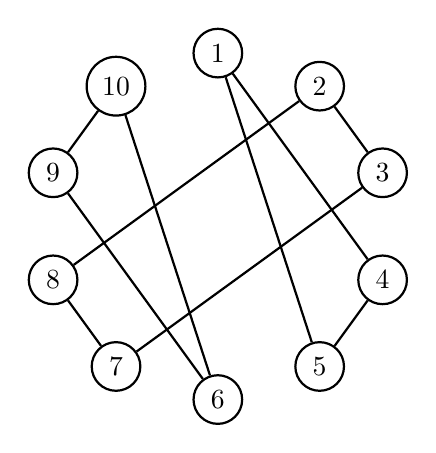
\begin{tikzpicture}[scale=0.6]
	\begin{scope}[every node/.style={circle,thick,draw}]
	\graph [clockwise] {
		subgraph I_n [n=10,name=A, radius=2.2cm]; 
		
		A 1 --[thick] A 4;
		A 4 --[thick] A 5; 
		A 5 --[thick] A 1;
		
		A 2 --[thick] A 3;
		A 3 --[thick] A 7;
		A 7 --[thick] A 8;
		A 8 --[thick] A 2;
		
		A 9 --[thick] A 10;
		A 10 --[thick] A 6; 
		A 6 --[thick] A 9;
		
	};
	\end{scope}
	\end{tikzpicture}
	\caption{A vertex-disjoint cycle cover}
	%\caption{Покрытие циклами без общих вершин}
	\label{image3}
\end{figure}

If $x$ and $y$ are undirected Hamiltonian cycles, then all vertices in the multigraph $x \cup y$ have degrees equal to $4$. Let $z$ be a vertex-disjoint cycle cover of $x \cup y$, then all the remaining edges form a graph $w = (x \cup y) \backslash z$ with all vertex degrees being equal to $2$. Thus, $w$ is also a vertex-disjoint cycle cover of $x \cup y$. %Если гамильтоновы циклы $x$ и $y$ не ориентированы, то все вершины в мультиграфе $x \cup y$ имеют степень $4$. Пусть $z$ --- покрытие $x \cup y$ циклами без общих вершин, тогда оставшиеся рёбра образуют граф $w = (x \cup y) \backslash z$, степени всех вершин которого равны $2$, а значит $w$ --- также является покрытием мультиграфа $x \cup y$ циклами без общих вершин.

If $x$ and $y$ are directed Hamiltonian tours, then all vertices in the multigraph $x \cup y$ have both indegrees and outdegrees equal to $2$. Let $z$ be a vertex-disjoint cycle cover of $x \cup y$, then in the digraph $w = (x \cup y) \backslash z$ all vertices have both indegrees and outdegrees equal to $1$. Thus, $w$ is also a vertex-disjoint cycle cover of $x \cup y$. %Если гамильтоновы контуры $x$ и $y$ ориентированы, то все вершины в мультиграфе $x \cup y$ имеют полустепени захода и исхода $2$. Пусть $z$ --- покрытие $x \cup y$ контурами без общих вершин, тогда в орграфе $w = (x \cup y) \backslash z$, каждая вершина имеет степень захода и исхода равную $1$, следовательно, $w$ --- также покрытие мультиграфа $x \cup y$ контурами без общих вершин.

Finding a vertex-disjoint cycle cover of both directed and undirected graph can be performed in polynomial time by a reduction to perfect matching \cite{Tutte}.
Let us recall that a perfect matching is a set of pairwise nonadjacent edges which matches all vertices of the graph. %Задача о построении покрытия циклами без общих вершин сводится к задаче построения совершенного паросочетания \cite{Tutte}. Напомним, что совершенным паросочетанием в графе называется множество попарно несмежных рёбер графа, в котором участвуют все вершины.
The procedures for directed and undirected graphs are somewhat different. We consider them separately. %Процедуры и алгоритмы для ориентированных и неориентированных графов несколько отличаются. Рассмотрим их по отдельности.

Let $x$ and $y$ be undirected Hamiltonian cycles. %Пусть $x$ и $y$ --- неориентированные циклы.
\begin{enumerate}
    \item [Step 1.] From the multigraph $x \cup y = G = (V, E)$, we construct a new graph $G' = (V', E')$. With each vertex $v \in V$ we associate a gadget $G_v$ that is a complete bipartite subgraph $K_{4,2}$ (note that the degree of $v$ equals 4) as it is shown in Fig.~\ref{image4}:
    %\item [Шаг 1.] По графу $x \cup y = G = (V, E)$ построим новый граф $G' = (V', E')$. Для этого каждой вершине $v \in V$ (степень вершины равна $4$) ставим в соответствие полный двудольный подграф $G_v = K_{4,2}$ и соединяем новые вершины рёбрами как показано на \autoref{image4}:
	\begin{itemize}
	    \item there are $4$ vertices in the outer part ($v_a$, $v_b$, $v_c$ and $v_d$) that correspond to $4$ edges incident to $v$ in $G$ (edges $A$, $B$, $C$, $D$); these vertices are connected with other gadgets; %\item $4$ вершины во внешней доле графа ($v_a$, $v_b$, $v_c$ и $v_d$) соответствуют 4 рёбрам, смежным с вершиной $v$ в оригинальном графе $G$ (рёбра $A$, $B$, $C$, $D$); они соединяются с соответствующими вершинами в других двудольных подграфах.
		\item there are $2$ vertices in the inner part ($v_1$ and $v_2$) that are connected only with the vertices of the outer part. %\item $2$ вершины во внутренней доле графа ($v_1$ и $v_2$) соединяются с каждой из $4$ вершин внешней доли.
	\end{itemize}
	\item [Step 2.] A perfect matching in $G'$ corresponds to a vertex-disjoint cycle cover in the original graph $G$.
	Indeed, a perfect matching has to cover both inner vertices $v_1$ and $v_2$. 
	Therefore, it includes exactly one edge of \{$(v_1,v_a)$, $(v_1,v_b)$, $(v_1,v_c)$, $(v_1,v_d)$\} and exactly one edge of $\{(v_2,v_a), (v_2,v_b), (v_2,v_c), (v_2,v_d)\}$.
	Both of these edges cover exactly two vertices of $\{v_a,v_b,v_c,v_d\}$.
	The other two vertices has to be covered by the edges that correspond to the edges of $G$ (Fig.~\ref{image5}). 
	We include these edges into $z$, then the degree of each vertex $v$ in the graph $z$ equals $2$, and thus, $z$ is a vertex-disjoint cycle cover of the multigraph $x \cup y$.
	%\item [Шаг 2.] Совершенному паросочетанию в графе $G'$ будет соответствовать покрытие циклами в исходном графе $G$. Действительно, требуется покрыть рёбрами внутренние вершины $v_1$ и $v_2$. Для этого в совершенное паросочетание будет включено ровно одно из рёбер \{$(v_1,v_a)$, $(v_1,v_b)$, $(v_1,v_c)$, $(v_1,v_d)$\} и ровно одно из рёбер $\{(v_2,v_a), (v_2,v_b), (v_2,v_c), (v_2,v_d)\}$. Эти два ребра покроют ровно две вершины из множества $\{v_a,v_b,v_c,v_d\}$. Две оставшиеся вершины будут покрыты двумя рёбрами из исходного графа (\autoref{image5}). Включим эти рёбра в подграф $z$, тогда степень каждой вершины $v$ в графе $z$ равна $2$, а значит это покрытие мультиграфа $x \cup y$ циклами без общих вершин.
\end{enumerate}

\begin{figure}[t]
	\centering
	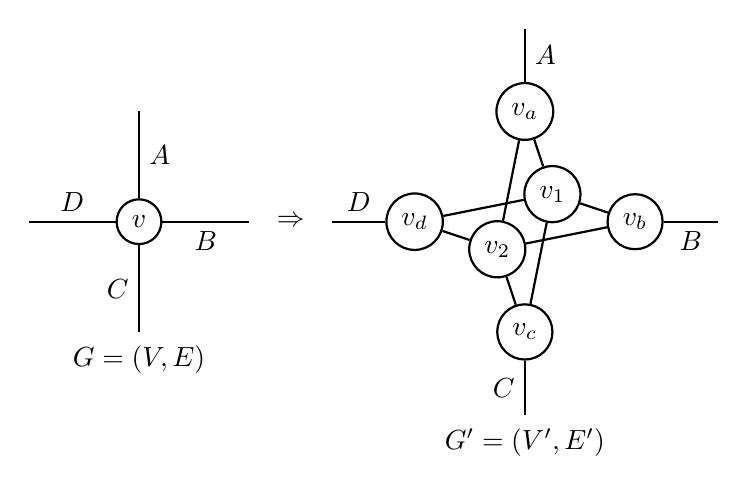
\begin{tikzpicture}[scale=0.7]
	\begin{scope}[every node/.style={circle,thick,draw}]
	\node (A) at (0,0) {$v$};
	\end{scope}
	\draw [thick] (A) -- node [right] {$A$} (0,2);
	\draw [thick] (A) -- node [below] {$B$} (2,0);
	\draw [thick] (A) -- node [left] {$C$} (0,-2);
	\draw [thick] (A) -- node [above] {$D$} (-2,0);
	\draw (0, -2.5) node{$G=(V,E)$};
	\node at (2.75,0) {$\Rightarrow$};
	\begin{scope}[xshift=7cm]
	\begin{scope}[every node/.style={circle,thick,draw}]
	\node (A) at (0,2) {$v_a$};
	\node (B) at (2,0) {$v_b$};
	\node (C) at (0,-2) {$v_c$};
	\node (D) at (-2,0) {$v_d$};
	\node (E) at (0.5,0.5) {$v_1$};
	\node (F) at (-0.5,-0.5) {$v_2$};
	\end{scope}
	\draw [thick] (E) edge (A);
	\draw [thick] (E) edge (B);
	\draw [thick] (E) edge (C);
	\draw [thick] (E) edge (D);
	\draw [thick] (F) edge (A);
	\draw [thick] (F) edge (B);
	\draw [thick] (F) edge (C);
	\draw [thick] (F) edge (D);
	\draw [thick] (A) -- node [right] {$A$} (0,3.5);
	\draw [thick] (B) -- node [below] {$B$} (3.5,0);
	\draw [thick] (C) -- node [left] {$C$} (0,-3.5);
	\draw [thick] (D) -- node [above] {$D$} (-3.5,0);
	\draw (0, -4) node{$G'=(V',E')$};
	\end{scope}
	\end{tikzpicture}
	\caption{Construction of the graph $G'$ for the symmetric problem}
	%\caption{Построение графа $G'$ для симметричной задачи}
	\label{image4}
\end{figure}

\begin{figure}[t]
	\centering
	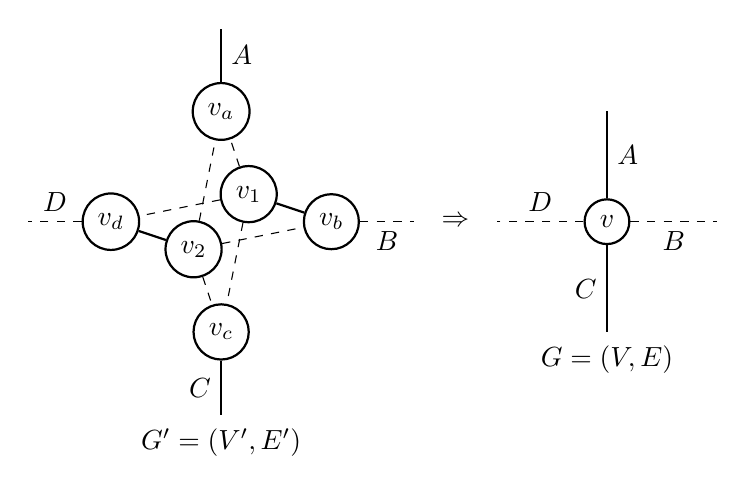
\begin{tikzpicture}[scale=0.7]
	\begin{scope}[every node/.style={circle,thick,draw}]
	\node (A) at (0,2) {$v_a$};
	\node (B) at (2,0) {$v_b$};
	\node (C) at (0,-2) {$v_c$};
	\node (D) at (-2,0) {$v_d$};
	\node (E) at (0.5,0.5) {$v_1$};
	\node (F) at (-0.5,-0.5) {$v_2$};
	\end{scope}
	\draw [dashed] (E) edge (A);
	\draw [thick] (E) edge (B);
	\draw [dashed] (E) edge (C);
	\draw [dashed] (E) edge (D);
	\draw [dashed] (F) edge (A);
	\draw [dashed] (F) edge (B);
	\draw [dashed] (F) edge (C);
	\draw [thick] (F) edge (D);
	\draw [thick] (A) -- node [right] {$A$} (0,3.5);
	\draw [dashed] (B) -- node [below] {$B$} (3.5,0);
	\draw [thick] (C) -- node [left] {$C$} (0,-3.5);
	\draw [dashed] (D) -- node [above] {$D$} (-3.5,0);
	\draw (0, -4) node{$G'=(V',E')$};
	
	\node at (4.25,0) {$\Rightarrow$};
	
	\begin{scope}[xshift=7cm]
	\begin{scope}[every node/.style={circle,thick,draw}]
	\node (A) at (0,0) {$v$};
	\end{scope}
	\draw [thick] (A) -- node [right] {$A$} (0,2);
	\draw [dashed] (A) -- node [below] {$B$} (2,0);
	\draw [thick] (A) -- node [left] {$C$} (0,-2);
	\draw [dashed] (A) -- node [above] {$D$} (-2,0);
	\draw (0, -2.5) node{$G=(V,E)$};

	\end{scope}
	\end{tikzpicture}
	\caption{A perfect matching in $G'$ and a vertex-disjoint cycle cover in $G$}
	%\caption{Совершенное паросочетание в $G'$ и покрытие циклами в $G$}
	\label{image5}
\end{figure}

A perfect matching in a general undirected graph can be found by Edmond's algorithm \cite{Edmonds} in $O(V^2 E)$ time or using Micali-Vazirani matching algorithm \cite{Micali} in $O(\sqrt{V} E)$ time. We have chosen Edmond's algorithm as a more simple one to implement. 
Note that replacing it with a more efficient Micali-Vazirani algorithm does not require changing the rest of the algorithm.
%Совершенное паросочетание в произвольном неориентированном графе может быть найдено алгоритмом Эдмондса \cite{Edmonds} за время $O(V^2 E)$ или алгоритмом Микали-Вазирани \cite{Micali} за время $O(\sqrt{V} E)$. Нами был выбран алгоритм Эдмондса как более простой в реализации. Отметим, что замена его на более эффективный алгоритм Микали-Вазирани не потребует изменения остальной части алгоритма.

Let $x$ and $y$ be directed Hamiltonian tours.
%Пусть $x$ и $y$ --- ориентированные контуры.
\begin{enumerate}
	\item [Step 1.] From the directed multigraph $x \cup y = D = (V, A)$, we construct a bipartite graph $D' = (L, R, E)$. With each vertex $v \in V$ we associate a pair of vertices $v_L \in L$ and $v_R \in R$, and with each edge $(u,v) \in A$ we associate a new edge $(u_L, v_R)$ in the bipartite graph $D'$ (Fig.~\ref{image6}). %\item [Шаг 1.] По ориентированному мультиграфу $x \cup y = D = (V, A)$ построим двудольный граф $D' = (L, R, E)$. Для этого каждой вершине $v \in V$ сопоставим пару вершин $v_L \in L$ и $v_R \in R$, а каждой дуге $(u, v) \in A$ --- ребро $(u_L, v_R)$ в двудольном графе $D'$ (\autoref{image6}).
	\item [Step 2.] A perfect matching in the bipartite graph $D'$ corresponds to a vertex-disjoint directed cycle cover in the original graph $D$.
	Indeed, every vertex of $D$ is a head of exactly one edge and a tail of exactly one edge of a perfect matching in $D'$ (Fig.~\ref{image7}). %\item [Шаг 2.] Совершенному паросочетанию в двудольном графе $D'$ будет соответствовать покрытие ориентированными циклами в исходном графе $D$. Действительно, после построения паросочетания получим, что из каждой вершины выходит ровно одно ребро, и в каждую вершину входит ровно одно ребро (\autoref{image7}).
\end{enumerate}

\begin{figure}[t]
	\centering
	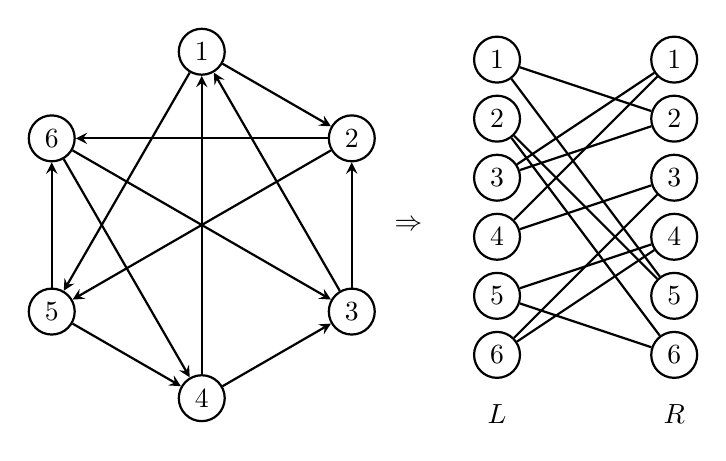
\begin{tikzpicture}[scale=0.75]
	\begin{scope}[every node/.style={circle,thick,draw,inner sep=3pt}]
	\graph [clockwise] {
		subgraph I_n [n=6,name=A, radius=2.2cm]; 
		
		A 1 --[->,>=stealth,thick] A 2;
		A 1 --[->,>=stealth,thick] A 5; 
		A 2 --[->,>=stealth,thick] A 5;
		A 2 --[->,>=stealth,thick] A 6;
		A 3 --[->,>=stealth,thick] A 1;
		A 3 --[->,>=stealth,thick] A 2;
		A 4 --[->,>=stealth,thick] A 1;
		A 4 --[->,>=stealth,thick] A 3;
		A 5 --[->,>=stealth,thick] A 4;
		A 5 --[->,>=stealth,thick] A 6;
		A 6 --[->,>=stealth,thick] A 3;
		A 6 --[->,>=stealth,thick] A 4;
	};
	\end{scope}
	\node at (3.5,0) {$\Rightarrow$};
	
	\begin{scope}[xshift=5cm,yshift=-2.2cm]
	\begin{scope}[every node/.style={circle,thick,draw,inner sep=3pt}]
	\node (A1) at (0,5) {1};
	\node (A2) at (0,4) {2};
	\node (A3) at (0,3) {3};
	\node (A4) at (0,2) {4};
	\node (A5) at (0,1) {5};
	\node (A6) at (0,0) {6};
	\node (B1) at (3,5) {1};
	\node (B2) at (3,4) {2};
	\node (B3) at (3,3) {3};
	\node (B4) at (3,2) {4};
	\node (B5) at (3,1) {5};
	\node (B6) at (3,0) {6};
	\end{scope}
	
	\node at (0,-1) {$L$};
	\node at (3,-1) {$R$};
	
	\draw [thick] (A1) edge (B2);
	\draw [thick] (A1) edge (B5);
	\draw [thick] (A2) edge (B5);
	\draw [thick] (A2) edge (B6);
	\draw [thick] (A3) edge (B1);
	\draw [thick] (A3) edge (B2);
	\draw [thick] (A4) edge (B1);
	\draw [thick] (A4) edge (B3);
	\draw [thick] (A5) edge (B4);
	\draw [thick] (A5) edge (B6);
	\draw [thick] (A6) edge (B3);
	\draw [thick] (A6) edge (B4);
	\end{scope}
	\end{tikzpicture}
	\caption{Construction of the bipatite graph $D'$ for the asymmetric problem}
	%\caption{Построение двудольного графа $D'$ для асимметричной задачи}
	\label{image6}
\end{figure}

\begin{figure}[t]
	\centering
	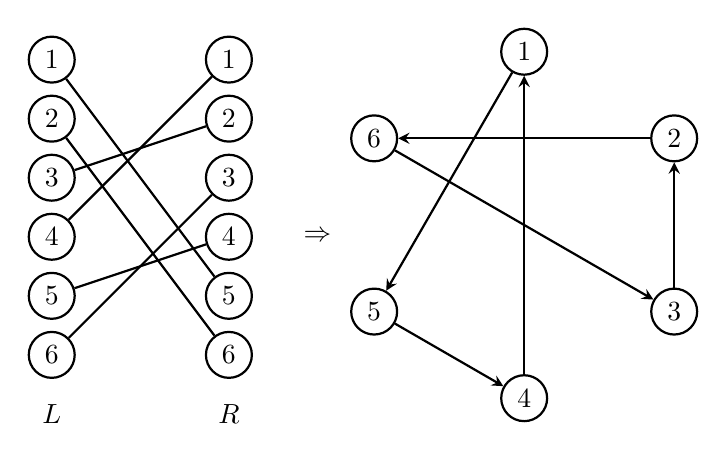
\begin{tikzpicture}[scale=0.75]
	\begin{scope}[every node/.style={circle,thick,draw,inner sep=3pt}]
	\node (A1) at (0,5) {1};
	\node (A2) at (0,4) {2};
	\node (A3) at (0,3) {3};
	\node (A4) at (0,2) {4};
	\node (A5) at (0,1) {5};
	\node (A6) at (0,0) {6};
	\node (B1) at (3,5) {1};
	\node (B2) at (3,4) {2};
	\node (B3) at (3,3) {3};
	\node (B4) at (3,2) {4};
	\node (B5) at (3,1) {5};
	\node (B6) at (3,0) {6};
	\end{scope}
	
	\node at (0,-1) {$L$};
	\node at (3,-1) {$R$};
	
	\draw [thick] (A1) edge (B5);
	\draw [thick] (A2) edge (B6);
	\draw [thick] (A3) edge (B2);
	\draw [thick] (A4) edge (B1);
	\draw [thick] (A5) edge (B4);
	\draw [thick] (A6) edge (B3);
	
	\node at (4.5,2) {$\Rightarrow$};
	
	\begin{scope}[xshift=8cm,yshift=2.2cm]
	\begin{scope}[every node/.style={circle,thick,draw,inner sep=3pt}]
	\graph [clockwise] {
		subgraph I_n [n=6,name=A, radius=2.2cm]; 
		
		A 1 --[->,>=stealth,thick] A 5; 
		A 2 --[->,>=stealth,thick] A 6;
		A 3 --[->,>=stealth,thick] A 2;
		A 4 --[->,>=stealth,thick] A 1;
		A 5 --[->,>=stealth,thick] A 4;
		A 6 --[->,>=stealth,thick] A 3;
	};
	\end{scope}
	\end{scope}
	\end{tikzpicture}
	\caption{A perfect matching in $D'$ corresponds to a vertex-disjoint cycle cover of $D$}
	%\caption{Совершенное паросочетанию $D'$ соответствует покрытие ориентированными циклами в $D$}
	\label{image7}
\end{figure}

A perfect matching in a bipartite graph can be found by Hopcroft–Karp algorithm \cite{Hopkroft} in $O(\sqrt{V} E)$ time. %Совершенное паросочетание может быть найдено алгоритмом Хопкрофта"=Карпа \cite{Hopkroft} за время $O(\sqrt{V} E)$.



\section{Generation of a neighbor candidate state} %\section{Переход к новому решению}
A process of constructing a neighbor candidate state is shown in Procedure~\ref{transit}. %Генерация нового состояния-кандидата приведена в процедуре~\ref{transit}.

\SetAlgorithmName{Algorithm}{Algorithm list}{} 
\SetAlgoCaptionSeparator{.} 
\DontPrintSemicolon
\SetKwProg{Proc}{Procedure}{}{End}
\SetKw{Return}{Return}
\begin{algorithm}[h]
	\label{transit}
	\caption{Constructing a neighbor candidate state}
	\SetKwData{z}{$z$}
	\SetKwData{w}{$w$}
	\SetKwData{numOfEdgesToFix}{$fixEdgesN$}
	\SetKwData{generateNeighbourCandidate}{$GenerateNeighbourCandidate$}
	\SetKwFunction{updateFixedEdges}{$UpdateFixedEdgesQueue$}
	\SetKwFunction{runBlossomAlgorithm}{$RunEdmondsAlgorithm$}
	\SetKwFunction{runHopcroftAlgorithm}{$RunHopcroftKarpAlgorithm$}
	\BlankLine
	
	\Proc{\generateNeighbourCandidate{\z, \w, \numOfEdgesToFix}}{
		\updateFixedEdges{\z, \w, \numOfEdgesToFix}\;

		\eIf{tours \z and \w are directed}{
			\runHopcroftAlgorithm{}\;
		} {
			\runBlossomAlgorithm{}\;
		}  

		\Return \z, \w\;
	}
\end{algorithm}

The algorithm receives as input the current state as the vertex-disjoint cycle covers $z$ and $w$, and the parameter $fixEdgesN$ that set the size of a queue of edges that are fixed in the graph $z$ and the corresponding perfect matching.
When this limit is exceeded, the first edge of the queue is deleted. %На вход подаётся текущее состояние в виде графов $z$ и $w$, а также параметр $\texttt{-{}-}fixEdgesN$, который описывает размер очереди рёбер, зафиксированных в графе $z$ и соответствующем паросочетании. При превышении этого лимита первое ребро очереди удаляется.

In order to find a neighbor candidate state we chose an edge of $w$ with endpoints in two different connected components of $z$ and add it to the queue of fixed edges (Fig.~\ref{image_exchange_rule}, fixed edges of $z$ are dashed, an edge of $w$ that is added to the queue is dashed dotted).
Such edge always exists due to the connectivity of the multigraph $x \cup y$ . 
If $z$ contains exactly one connected component, then the graphs $z$ and $w$ can be swapped. 
The idea of this procedure is to reduce the number of connected components in $z$ and $w$.
The neighbor candidate state is constructed by the perfect matching algorithms with fixed edges forming the initial matching.
%При генерации нового состояния-кандидата в очередь добавляется ребро графа $w$, которое соединяет две компоненты связности графа $z$. Такое ребро обязательно найдётся в силу связности мультиграфа $x \cup y$ (\autoref{image_exchange_rule}). Если в графе $z$ всего одна компонента связности, то графы $z$ и $w$ меняются местами. Рёбра выбираются таким образом, чтобы стремиться к уменьшению компонент связности в покрытии циклами. Новое состояние-кандидат пересчитывает алгоритмами построения совершенного паросочетания с учётом очереди из фиксированных рёбер.

\begin {figure} [t]
\centering
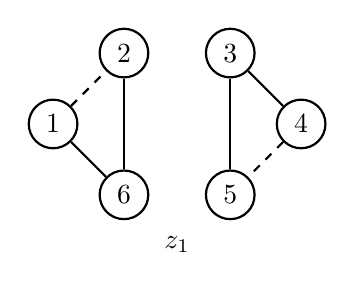
\begin{tikzpicture}[scale=0.9]
\begin{scope}[every node/.style={circle,thick,draw}]
\node (A) at (0,0) {1};
\node (B) at (1,1) {2};
\node (C) at (2.5,1) {3};
\node (D) at (3.5,0) {4};
\node (E) at (2.5,-1) {5};
\node (F) at (1,-1) {6};
\end{scope}
\draw [thick, dashed] (A) edge (B);
\draw [thick] (B) edge (F);
\draw [thick] (F) edge (A);
\draw [thick] (C) edge (D);
\draw [thick, dashed] (D) edge (E);
\draw [thick] (E) edge (C);
\draw (1.75, -1.7) node{$z_{1}$};
\end{tikzpicture}
\hspace*{6mm}
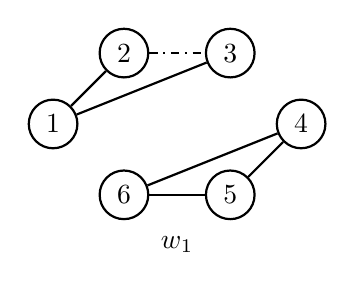
\begin{tikzpicture}[scale=0.9]
\begin{scope}[every node/.style={circle,thick,draw}]
\node (A) at (0,0) {1};
\node (B) at (1,1) {2};
\node (C) at (2.5,1) {3};
\node (D) at (3.5,0) {4};
\node (E) at (2.5,-1) {5};
\node (F) at (1,-1) {6};
\end{scope}
\draw [thick] (A) edge (B);
\draw [thick, dashdotted] (B) edge (C);
\draw [thick] (C) edge (A);
\draw [thick] (D) edge (E);
\draw [thick] (E) edge (F);
\draw [thick] (F) edge (D);
\draw (1.75, -1.7) node{$w_{1}$};
\end{tikzpicture}
\\
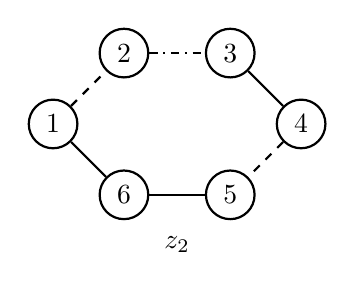
\begin{tikzpicture}[scale=0.9]
\begin{scope}[every node/.style={circle,thick,draw}]
\node (A) at (0,0) {1};
\node (B) at (1,1) {2};
\node (C) at (2.5,1) {3};
\node (D) at (3.5,0) {4};
\node (E) at (2.5,-1) {5};
\node (F) at (1,-1) {6};
\end{scope}
\draw [thick, dashed] (A) edge (B);
\draw [thick, dashdotted] (B) edge (C);
\draw [thick] (C) edge (D);
\draw [thick, dashed] (D) edge (E);
\draw [thick] (E) edge (F);
\draw [thick] (F) edge (A);
\draw (1.75, -1.7) node{$z_{2}$};
\end{tikzpicture}
\hspace*{6mm}
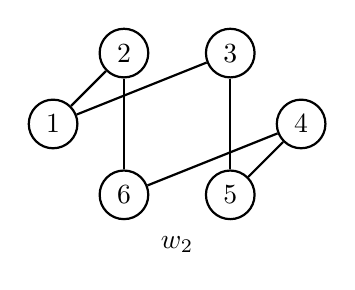
\begin{tikzpicture}[scale=0.9]
\begin{scope}[every node/.style={circle,thick,draw}]
\node (A) at (0,0) {1};
\node (B) at (1,1) {2};
\node (C) at (2.5,1) {3};
\node (D) at (3.5,0) {4};
\node (E) at (2.5,-1) {5};
\node (F) at (1,-1) {6};
\end{scope}
\draw [thick] (A) edge (B);
\draw [thick] (B) edge (F);
\draw [thick] (F) edge (D);
\draw [thick] (D) edge (E);
\draw [thick] (E) edge (C);
\draw [thick] (C) edge (A);
\draw (1.75, -1.7) node{$w_{2}$};
\end{tikzpicture}
\caption {Generation of a neighbor candidate state}
%\caption {Переход к новому решению}
\label {image_exchange_rule}
\end{figure}


\section{Cooling schedule} %\section{Функция понижения температуры} 

If a neighbor candidate state has two complementary Hamiltonian tours different from $x$ and $y$ (or any two complementary Hamiltonian tours, if the input is a $2/4$-regular graph), then the algorithm successfully stops and returns a solution.
%Следующий шаг алгоритма~--- проверка остановки. Если при генерации состояния-кандидата на текущем шаге были получены $2$ гамильтоновых цикла (контура), отличные от исходных, программа успешно останавливает работу и выводит решение. В случае, если исходным форматом входных данных был выбран объединённый $2/4$"~регулярный граф, для завершения требуется получить разбиение на любые $2$ гамильтоновых цикла (контура).

Otherwise, the energy function is calculated for a neighbor candidate state.
We have chosen the following function
(Procedure~\ref{calcEnergy}): (number of connected components in $z$) + (number of connected components in $w$).

\SetAlgorithmName{Algorithm}{Algorithm list}{} 
\SetAlgoCaptionSeparator{.} 
\DontPrintSemicolon
\SetKwProg{Proc}{Procedure}{}{End}
\SetKw{Return}{Return}
\begin{algorithm}[h]
	\label{calcEnergy}
	\caption{Energy function}
	\SetKwData{z}{$z$}
	\SetKwData{w}{$w$}
	\SetKwData{stateCandidate}{$stateCandidate$}
	\SetKwData{calculateEnergy}{$CalculateEnergy$}
	\SetKwFunction{countComponents}{$CountComponents$}
	
	\BlankLine
	\Proc{\calculateEnergy{\z, \w}}{
		\Return \countComponents{\z} + \countComponents{\w}\;
	}
	\BlankLine
\end{algorithm}

At each step of the algorithm the candidate states correspond to two vertex-disjoint cycle covers $z$ and $w$. Therefore, if the total number of connected components in $z$ and $w$ is equal to $2$, then $z$ and $w$ are Hamiltonian tours. %Иначе происходит подсчёт энергии (значения целевой функции) для состояния-кандидата. В качестве целевой функции для оптимизации была взята следующая (процедура~\ref{calcEnergy}): (число компонент связности в графе $z$) + (число компонент связности в графе $w$). На каждом шаге алгоритма состояния-кандидаты соответствуют двум покрытиям циклами $z$ и $w$. Следовательно, если число компонент связности в графах $z$ и $w$ равно одному, то это гамильтоновы циклы (контуры).



If the energy function has decreased compared to the previous state, then we accept a transition to the neighbor candidate state.  %Если подсчитанная энергия уменьшилась по сравнению с предыдущим состоянием, то переход в новое состояние"=кандидат однозначно осуществляется.

If the energy function has not decreased, then we make a transition with probability
\[P = e^{-\frac{currE - candE}{T}},\]
where $T$ is the current temperature, $currE$ is the current energy value, and $candE$ is the energy of the considered neighbor candidate state.
Such transition is necessary to avoid the problem of falling into the local minimum. %Если подсчитанная энергия не уменьшилась, то переход в состояние осуществляется с определенной вероятностью $P$. Такой переход нужен для того, чтобы избежать проблемы попадания в локальный минимум.

The current temperature gradually decreases from $initT$ to $0$, and its function depends on the initial temperature $initT$ and the index of the current iteration $k$ (Procedure \ref{tempdecr}).

\SetAlgorithmName{Algorithm}{Algorithm list}{} 
\SetAlgoCaptionSeparator{.} 
\DontPrintSemicolon
\SetKwProg{Proc}{Procedure}{}{End}
\SetKw{Return}{Return}
\begin{algorithm}[!htbp]
	\label{tempdecr}
	\caption{Cooling schedule}
	\SetKwData{k}{$k$}
	\SetKwData{startTemp}{$initT$}
	\SetKwData{coolingSchedule}{$CoolingSchedule$}
	
	\BlankLine
	\Proc{\coolingSchedule{\k}}{
		\Return  \startTemp / \k\;
	}
	\BlankLine
\end{algorithm}

    %getTransitionProbability(E, T) {
    %    return Math.exp(-E / T);
    %}

    %decreaseTemperature(initialTemperature, k) {
    %    return initialTemperature / k;
    %}



\section{Experiments} %\section{Приложение и тесты}

The algorithm to test vertex adjacencies in the polytopes $\TSP(n)$ and $\ATSP(n)$ was implemented as a console application with different input parameters. Some of them are described below: %Программа может быть запущена с разным набором параметров. Далее приводится описание некоторых возможных параметров запуска:

\begin{description}
    \item [\texttt{-{}-}N]~--- number of vertices in the input graph/tour; %число вершин во входном графе/цикле
    \item [\texttt{-{}-}times]~--- number of times to run the algorithm; %число тестов, для которых запускается алгоритм
    
    \item [\texttt{-{}-}iterN]~--- number of iterations in the simulated annealing algorithm; %число шагов в алгоритме имитации отжига
    
    \item [\texttt{-{}-}stateCandidate=random|match]~--- how to generate a neighbor candidate state: %способ генерации состояния"=кандидата в агоритме имитации отжига:
    \begin{enumerate}
        \item [\textit{random}]: random exchange of edges between tours %случайный обмен рёбрами
        \item [\textit{match}]: constructing a vertex-disjoint cycle cover and a perfect matching; %пересчёт циклов через паросочетания
    \end{enumerate}
    
    \item [\texttt{-{}-}exEdgesN]~--- number of edges to randomly exchange between tours (used only for \texttt{-{}-}stateCandidate=random); %число рёбер для случайного обмена между циклами (только для \texttt{-{}-}stateCandidate=random)
    
    \item [\texttt{-{}-}ansN]~--- multistart: number of repeatedly runs of the algorithm (used only for \texttt{-{}-}stateCandidate=random); % мультистарт: число решений, генерируемых одновременно (только для \texttt{-{}-}stateCandidate=random)
    
    \item [\texttt{-{}-}fixEdgesN]~--- the size of a queue of edges that can be fixed in the initial matching (used only for \texttt{-{}-}stateCandidate=match). %максимальное число зафиксированных ребер, добавленных в очередь, для формирования начального паросочетания (только для \texttt{-{}-}stateCandidate=match)
\end{description}

%The results of testing with different input parameters are given below.
We tested the algorithm on random directed and undirected Hamiltonian tours, and also on directed and undirected pyramidal tours.
 % Ниже приведены результаты тестирования программы для различных входных параметров. Тестирование проходило на ориентированных и неориентированных случайных гамильтоновых циклах, также на ориентированных и неориентированных пирамидальных циклах.

A Hamiltonian tour %Гамильтонов цикл 
\[\tau = (1, i_1, i_2, \ldots, i_r, n, j_1, j_2, \ldots, j_{n-r-2})\] 
is called \textit{pyramidal} if %называется пирамидальным, если 
\[i_1 < i_2 < \ldots < i_r \text{ and } j_1 > j_2 > \ldots > j_{n-r-2}.\]

We chose pyramidal tours for experiments since for them the vertex adjacencies in the corresponding polytopes can be easily verified.
In particular, the following problem: given two pyramidal tours $x$ and $y$, is it possible to construct two complementary tours $z$ and $w$ from the edges of $x$ and $y$, can be solved in linear time \cite{Bondarenko-Nikolaev-2017,Bondarenko-Nikolaev-2018}.
Thus, we run the algorithm on pyramidal tours, for which it is known that the sufficient condition of Lemma~\ref{lemma_nonadjacency} is satisfied.
This allows us to estimate the error percentage when the algorithm could not find complementary tours that are guaranteed to exist. %Пирамидальные маршруты коммивояжёра были выбраны потому, что для них известны легко проверяемые критерий смежности вершин в соответствующих многогранниках. В частности, следующая задача: заданы два пирамидальных цикла (контура) $x$ и $y$, можно ли из их рёбер собрать два дополнительных цикла (контура) $z$ и $w$, разрешима за линейное время \cite{Bondarenko-Nikolaev-2017,Bondarenko-Nikolaev-2018}. Алгоритм тестировался на пирамидальных циклах (контурах), для которых гарантированно известно, что достаточное условие леммы~\ref{lemma_nonadjacency} выполнено. Это позволило оценить процент ошибки, когда алгоритм не смог найти дополнительные циклы, которые согласно критерию должны существовать.

The results of the tests for undirected pyramidal tours are presented in Table~\ref{tabl:table1} (Edmond's algorithm is used). %В таблице \ref{tabl:table1} приведены результаты тестирования программы для неориентированных пирамидальных циклов (используется алгоритм Эдмондса). 
The algorithm was run with the number of iterations $iterN = 8000$ and the number of fixed edges $fixEdgesN = \lfloor N/3 \rfloor$. %Алгоритм был запущен с числом итераций $\texttt{-{}-}iterN = 8000$ и числом фиксированных рёбер $\texttt{-{}-}fixEdgesN = [N/3]$. 
In the previous version of the program~\cite{Kozlova} a different method to generate neighbor candidate state was implemented~--- the exchange of random edges between two subgraphs $z$ and $w$. Its results are also shown in the table for comparison. For the exchange of random edges the following input parameters were used: the number of iterations $iterN = 50000$, the number of multistart attempts $ansN = 5$ and the number of edges to exchange $exEdgesN = 3$. %В предыдущей версии программы \cite{Kozlova} для генерации состояния-канди\-дата был реализован алгоритм случайного обмена рёбер между двумя подграфами $z$ и $w$, его результаты работы также представлены в таблице для сравнения. Для запуска случайного обмена были использованы следующие входные параметры: число итераций $\texttt{-{}-}iterN = 50000$, число запусков процедуры $\texttt{-{}-}ansN = 5$ и число рёбер для обмена $\texttt{-{}-}exEdgesN = 3$.

\begin{table}[t]
	\centering
	\caption{Results for undirected pyramidal tours with number of tests $times = 50$}	\label{tabl:table1}
	\begin{tabular}{|*{9}{c|}}
		\hline
		& \multicolumn{4}{c|}{Exchange of random edges} &  \multicolumn{4}{c|}{Reconstructing with perfect matching} \\ 
		%& \multicolumn{4}{c|}{Случайный обмен рёбер} &  \multicolumn{4}{c|}{Пересчёт через паросочетания} \\ 
		\hline
		& Tours & Tours &  &  & Tours & Tours &  & \\
		& are not & are & Average & Accuracy, & are not & are & Average & Accuracy,\\
		& found, & found, & time, & \%, & found, & found, & time, & \%, \\
		N & $TNF_{avg}$ & $TF_{avg}$ & $T_{avg}$ & $Acc$ & $TNF_{avg}$ & $TF_{avg}$ & $T_{avg}$ & $Acc$ \\ 
		%& Циклы &  &  &  & Циклы &  &  & \\
		%& не & Циклы & Среднее & Точность, & не & Циклы & Среднее & Точность,\\
		%& найдены, & найдены, & время, & \%, & найдены, & найдены, & время, & \%, \\
		%N & $TNF_{avg}$ & $TF_{avg}$ & $T_{avg}$ & Accuracy & $TNF_{avg}$ & $TF_{avg}$ & $T_{avg}$ & Accuracy \\ 
		\hline
		8 & $-$ & 9,84 & 9,84 & 100 & $-$ & 5,57 & 5,57 & 100 \\ 
		\hline
		16 & 5066,57 & 382,79 & 851,17 & 90 & $-$ & 22,08 & 22,08 & 100 \\ 
		\hline
		24 & 6549,75 & 1403,32 & 5005,82 & 30 & 9096,65 & 33,34 & 214,61 & 98 \\ 
		\hline
		32 & 7832,24 & 1330,37 & 7312,09 & 8 & $-$ & 224,93 & 224,93 & 100 \\ 
		\hline
		40 & 10035,64 & 2351,53 & 9728,28 & 4 & 18656,05 & 610,26 & 971,18 & 98 \\
		\hline
		48 & 13455,39 & $-$ & 13455,39 & 0 & 27695,76 & 978,18 & 3649,94 & 90 \\
		\hline
		64 & 16243,99 & 108,64 & 15921,28 & 2 & 48377,16 & 988,05 & 12361,43 & 76 \\ 
		\hline
		96 &  \multicolumn{4}{c|}{} & 98409,5 & 12293,68 & 53629,27 & 52 \\ 
		\cline{1-1}\cline{6-9}
		128 &  \multicolumn{4}{c|}{\_}  & 158485,17 & 21982,49 & 120264,4 & 28 \\ 
		\cline{1-1}\cline{6-9}
		192 &  \multicolumn{4}{c|}{}  & 334841,38 & 26165,54 & 297800,28 & 12 \\ 
		%\cline{1-1}\cline{6-9}
		%256 &  \multicolumn{4}{c|}{}  &  &  &  &  \\ 
		\hline
	\end{tabular}
\end{table} 

Note that compared to the exchange of random edges, both the accuracy of the algorithm and the size of solved problems have increased. The accuracy can also be adjusted by increasing the number of iterations or changing the maximum number of fixed edges in the queue. %Видно, что по сравнению со случайным обменом рёбрами возросла точность работы, и размер решаемых задач. Точность также можно регулировать, увеличивая число итераций или изменяя значение фиксированных рёбер в очереди.


The results of the tests for directed pyramidal tours and the Hopcroft-Karp algorithm are presented in Table~\ref{tabl:table2}.
The input parameters are similar to the case with undirected tours. 
Here, for almost all considered sizes of test graphs, the algorithm works with the accuracy of $100\%$, which is a very good result. %Далее были проведены тесты для ориентированных пирамидальных циклов и алгоритма Хопкрофта-Карпа (\autoref{tabl:table2}) с числовыми параметрами, аналогичными запуску на неориентированных циклах. Здесь практически для всех рассмотренных размеров тестовых графов алгоритм работает с точностью $100\%$, что является очень хорошим результатом.

\begin{table}[t]
	\centering
	\caption{\label{tabl:table2}Results for directed pyramidal tours (Hopcroft-Karp algorithm), with the number of tests $times = 50$ and number of fixed edges $fixEdgesN = [N/3]$}
	\begin{tabular}{|*{5}{c|}}
		\hline
		& Tours & Tours & Average & \\
		& are not found, & are found, & time, & Accuracy, \%, \\
		N & $TNF_{avg}$ & $TF_{avg}$ & $T_{avg}$ & $Acc$ \\ 
		%& Циклы & Циклы & Среднее & \\
		%& не найдены, & найдены, & время, & Точность, \%, \\
		%N & $TNF_{avg}$ & $TF_{avg}$ & $T_{avg}$ & Accuracy \\ 
		\hline
		8 & $-$ & 2,27 & 2,27 & 100 \\ 
		\hline
		16 & $-$ & 5,03 & 5,03 & 100 \\ 
		\hline
		24 & $-$ & 19,75 & 19,75 & 100 \\ 
		\hline
		32 & $-$ & 19,14 & 19,14 & 100 \\ 
		\hline
		40 & $-$ & 40,89 & 40,89 & 100 \\ 
		\hline
		48 & $-$ & 95,38 & 95,38 & 100 \\
		\hline
		64 & $-$ & 689,20 & 689,20 & 100 \\
		\hline
		96 & $-$ & 330,21 & 330,21 & 100 \\
		\hline
		128 & 129532,21 & 4514,36 & 9515,07 & 96 \\
		\hline
		192 & 242480,51 & 15783,70 & 70190,93 & 76 \\
		%\hline
		%256 &  &  &  &  \\
		\hline
	\end{tabular}
\end{table}

Finally, Table~\ref{tabl:table3} shows the test results for random directed and undirected Hamiltonian tours. From the table it can be concluded that for random tours the algorithm works even faster than for pyramidal tours.
Note that for undirected graphs the algorithm finds complementary tours more often than for directed graphs. This is due to the fact that $1$-skeleton of the asymmetric traveling salesperson polytope is generally much more dense than $1$-skeleton of the symmetric polytope. For example, the diameter of $1$-skeleton of $\ATSP(n)$ is $2$ \cite{Padberg}, while the best known upper bound for the diameter of $1$-skeleton of $\TSP(n)$ is $4$ \cite{Rispoli}.
Besides, for undirected cycles, the algorithm was able to find a solution for almost all cases. 
We can conclude that for the symmetric traveling salesperson polytope $\TSP(n)$ two random vertices are not adjacent with a very high probability. %Наконец, в таблице \ref{tabl:table3} приведены результаты запуска процедуры для случайных ориентированных и неориентированных гамильтоновых циклах. Из таблицы можно заметить, что для случайных циклов алгоритм работает достаточно быстро, даже быстрее чем на пирамидальных. Кроме того, для неориентированных циклов он сумел найти решение практически для всех тестовых случаев. Можно сделать вывод, что для симметричного многогранника задачи коммивояжёра $\TSP(n)$ две случайных вершины с высокой вероятностью будут не смежны.

%Отметим, что для неориентированных графов алгоритм находит дополнительные циклы намного чаще, чем для ориентированных контуров. Это связано с тем, что полиэдральный граф асимметричной задачи коммивояжёра в целом является намного более плотным, чем полиэдральный граф симметричной задачи. Так, диаметр полиэдрального графа $\ATSP(n)$ равен $2$ \cite{Padberg}, а лучшая известная верхняя оценка на диаметр полиэдрального графа $\TSP(n)$ составляет $4$ \cite{Rispoli}.

The largest instance that was solved by the algorithm had random Hamiltonian tours on $4096$ vertices and required $1\,530\,682$ ms.
However, due to the long waiting time for several tests, we limited the presented experiments to tours of size under $200$ vertices.

\begin{table}[!htbp]
\centering
\caption{%\label{tabl:table3}
\label{tabl:table3}Results for random Hamiltonian tours with the number of tests $times = 50$}
\begin{tabular}{|*{9}{c|}}
\hline
& \multicolumn{4}{c|}{Undirected tours} &  \multicolumn{4}{c|}{Directed tours} \\ 
%& \multicolumn{4}{c|}{Неориентированные циклы} &  \multicolumn{4}{c|}{Ориентированные контуры} \\ 
\hline
  & Tours & Tours &  & Percentage & Tours & Tours &  & Percentage \\
  & are not & are & Average & of found & are not & are & Average & of found \\
  & found, & found, & time, & tours, & found, & found, & time, & tours, \\
  %&  &  &  & Доля &  &  &  & Доля \\
  %& Циклы &  &  & найден"~ & Циклы &  &  & найден"~ \\
  %& не & Циклы & Среднее & ных & не & Циклы & Среднее & ных \\
  %& найдены, & найдены, & время, & циклов & найдены, & найдены, & время, & циклов \\
N & $TNF_{avg}$ & $TF_{avg}$ & $T_{avg}$ & \% & $TNF_{avg}$ & $TF_{avg}$ & $T_{avg}$ & \% \\ 
\hline
8 & 1604,66 & 15,02 & 491,91 & 30 & 3118,99 & 4,05 & 2682,90 & 14 \\ 
\hline
16 & $-$ & 13,76 & 13,756 & 100 & 6799,17 & 4,71 & 4624,95 & 32 \\ 
\hline
24 & $-$ & 28,52 & 28,52 & 100 & 10594,29 & 9,38 & 8265,61 & 22 \\ 
\hline
32 & $-$ & 46,64 & 46,64 & 100 & 14764,29 & 39,19 & 10052,26 & 32 \\ 
\hline
40 & $-$ & 75,27 & 75,27 & 100 & 19184,31 & 19,33 & 15734,62 & 18 \\ 
\hline
48 & $-$ & 87,86 & 87,86 & 100 & 25214,48 & 142,08 & 19197,11 & 24 \\ 
\hline
64 & $-$ & 235,37 & 235,37 & 100 & 38886,56 & 238,95 & 29611,13 & 24 \\ 
\hline
96 & $-$ & 481,37 & 481,37 & 100 & 74654,25 & 1150,20 & 61423,52 & 18 \\ 
\hline
128 & $-$ & 827,42 & 827,42 & 100 & 121790,32 & 1851,29 & 95403,73 & 22 \\ 
\hline
192 & $-$ & 4064,84 & 4064,84 & 100 & 252321,67 & 8979,84 & 213386,98 & 16 \\ 
%\hline
%256 &  &  &  &  & &  &  & \\ 
\hline
\end{tabular}
\end{table}


\section{Conclusion} 

The construction and study of $1$-skeletons of the polytopes associated with intractable problems is of interest for the development and analysis of combinatorial algorithms.
However, for such problems as the traveling salesperson even determining whether two vertices are adjacent or not is an NP-complete problem.
This paper proposes an original heuristic approach based on simulated annealing to verify vertex adjacencies in $1$-skeleton of the traveling salesperson polytope.
The algorithm has a one-sided error: the answer ``not adjacent'' is always correct, while the answer ``probably adjacent'' leaves the possibility that the vertices actually are not adjacent.
The algorithm showed good practical results during the experiments.
%Построение и исследование полиэдральных графов многогранников труднорешаемых задач имеет большое значение для разработки и анализа комбинаторных алгоритмов. Однако для таких задач как коммивояжёр уже проверка смежности вершин в полиэдральном графе является NP-полной задачей. В данной статье предлагается оригинальный эвристический подход на основе имитации отжига для решения геометрической задачи проверки смежности вершин в полиэдральном графе задачи коммивояжёра. Алгоритм является алгоритмом с односторонней ошибкой: ответ <<не смежны>> всегда корректен, ответ <<возможно не смежны>> оставляет задачу открытой. При тестировании алгоритм показал неплохие практические результаты.


\subsubsection*{Acknowledgments.}%.\subsubsection*{Благодарности.}
The research is supported by the grant of the President of the Russian Federation MK-2620.2018.1. %Работа выполнена при поддержке гранта Президента Российской Федерации МК-2620.2018.1.

% ---- Bibliography ----
%
% BibTeX users should specify bibliography style 'splncs04'.
% References will then be sorted and formatted in the correct style.
%
% \bibliographystyle{splncs04}
% \bibliography{mybibliography}
%

\bibliographystyle{splncs04}
\begin{thebibliography}{99}
	
	\bibitem{Ageev}
	Ageev, A.A., Pyatkin, A.V.: 
	A 2-approximation algorithm for the metric 2-peripatetic salesman problem.
	In: {\em 5th International Workshop on Approximation and Online Algorithms, WAOA 2007, LNCS 4927}, 103--115, 2016.
	\doi{10.1007/978-3-540-77918-6\_9}.
	
	
	\bibitem {Aguilera}
	Aguilera, N.E., Katz, R.D., Tolomei, P.B.: 
	Vertex adjacencies in the set covering polyhedron. 
	{\em Discrete Appl. Math.} {\bf 218}, 40--56 (2017).
	\doi{10.1016/j.dam.2016.10.024}.
	
	
	\bibitem {Balinski}
	Balinski, M.L.: 
	Signature methods for the assignment problem.
	{\em Oper. Res.} {\bf 33} (3), 527--536 (1985).
	\doi{10.1287/opre.33.3.527}.
	
	
	\bibitem {Baburin}
	Baburin, A.E., Della Croce, F., Gimadi, E.K., Glazkov, Y.V., Paschos, V.Th.: 
	Approximation algorithms for the 2-peripatetic salesman problem with edge weights 1 and 2.
	{\em Discrete Appl. Math.} {\bf 157}, 1988--1992 (2009).
	\doi{10.1016/j.dam.2008.06.025}.
	
	
	\bibitem {Bondarenko}
	Bondarenko, V.A.:
	Nonpolynomial lower bounds for the complexity of the traveling salesman problem in a class of algorithms.
	{\em Autom. Rem. Contr.} {\bf 44}, 1137--1142 (1983).
	
	
	\bibitem{Bondarenko-Maksimenko}
	Bondarenko, V.A., Maksimenko, A.N.:
	Geometricheskie konstruktsii i slozhnost' v kombinatornoy optimizatsii (Geometric constructions and complexity in combinatorial optimization), LKI, Moscow, 2008 [Russian].
	
	
	\bibitem{Bondarenko-Nikolaev-2016}
	Bondarenko, V.A., Nikolaev, A.V.:
	On Graphs of the Cone Decompositions for the Min-Cut and Max-Cut Problems,
	{\em Int. J. Math. Sci.,} {\bf 2016}, Article ID 7863650, 6~p (2016).
	\doi{10.1155/2016/7863650}.
	
	
	\bibitem{Bondarenko-Nikolaev-2017}
	Bondarenko, V.A., Nikolaev, A.V.:
	Some properties of the skeleton of the pyramidal tours polytope.
	{\em Electron. Notes Discrete Math.} {\bf 61}, 131--137 (2017).
	\doi{10.1016/j.endm.2017.06.030}.
	
	
	\bibitem {Bondarenko-Nikolaev-2018}
	Bondarenko, V.A., Nikolaev, A.V.:
	On the Skeleton of the Polytope of Pyramidal Tours.
	{\em J. Appl. Ind. Math.} {\bf 12}, 9-18 (2018).
	\doi{10.1134/S1990478918010027}.
	
	
%	\bibitem{Burkard}
%	Burkard, R.E., Deineko, V.G., Van Dal, R., Van der Veen, J.A.A., Woeginger, G.J.:
%	Well-Solvable Special Cases of the Traveling Salesman Problem: A Survey.
%	{\em SIAM Rev.}, {\bf 40}, 496--546 (1998).
%	\doi{10.1137/S0036144596297514}.
	
	
	\bibitem {Chegireddy}
	Chegireddy, C.R., Hamacher, H.W.: 
	Algorithms for finding K-best perfect matchings. 
	{\em Discrete Appl. Math.} {\bf 18}, 155--165 (1987).
	\doi{10.1016/0166-218X(87)90017-5}
	
	
	\bibitem {Combarro}
	Combarro, E.F., Miranda, P.:
	Adjacency on the order polytope with applications to the theory of fuzzy measures.
	{\em Fuzzy Set. Syst.} {\bf 161}, 619--641 (2010).
	\doi{10.1016/j.fss.2009.05.004}.
	
	
	\bibitem {DeKort}
	De Kort, J.B.J.M.:
	Bounds for the Symmetric 2-Peripatetic Salesman Problem.
	{\em Optim.} {\bf 23}, 357--367 (1992).
	\doi{10.1080/02331939208843770}.
	
	
	\bibitem {Edmonds}
	Edmonds, J.:
	Paths, trees, and flowers.
	{\em Can. J. Math.} {\bf 17}, 449--467 (1965).
	\doi{10.4153/CJM-1965-045-4}.
		
	
	\bibitem {Fiorini}
	Fiorini, S., Massar, S., Pokutta, S., Tiwary, H.R., De Wolf, R.: 
	Exponential Lower Bounds for Polytopes in Combinatorial Optimization.
	{\em J. ACM} {\bf 62}, Article No. 17 (2015).
	\doi{10.1145/2716307}.
	
	
	\bibitem {Gabow}
	Gabow, H.N.:
	Two algorithms for generating weighted spanning trees in order.
	{\em SIAM J. Comput.} {\bf 6}, 139--150 (1977).
	\doi{10.1137/0206011}.
	
	
	\bibitem {Glebov}
	Glebov, A.N., Zambalaeva, D.Z.: 
	A polynomial algorithm with approximation ratio 7/9 for the maximum two peripatetic salesmen problem.
	{\em J. Appl. Ind. Math.} {\bf 6}, 69--89 (2012).
	\doi{10.1134/S1990478912010085}.
	
	
	\bibitem {Grotschel}
	Gr\"{o}tschel, M.; Padberg, M.:
	Polyhedral theory. In: \textit{The Traveling Salesman Problem: A Guided Tour of Combinatorial Optimization}, E.\,Lawler, J.\,K.\,Lenstra, A.\,Rinnooy Kan, and
	D.\,Shmoys, eds., pp.~251--305, John Wiley, Chichester, 1985.
	
	
	\bibitem{Hopkroft}
	Hopcroft, J.E., Karp, R.M.:
	An $n^{5 \slash 2}$ algorithm for maximum matchings in bipartite graphs.
	{\em SIAM J. Comp.} {\bf 2} (4), 225--231 (1973).
	\doi{10.1137/0202019}.
	
		
	\bibitem{Kirkpatrick}
	Kirkpatrick, S, Gelatt, C.D., Vecchi, M.P.: 
	Optimization by simulated annealing.
	{\em Science.} {\bf 220} (4598), 671--680 (1983).
	\doi{10.1126/science.220.4598.671}.
	
	
	\bibitem{Kozlova}
	Kozlova, A.P., Nikolaev, A.V.:
	Proverka smezhnosti vershin mnogogrannika zadachi kommivoyazhyora (Verification of vertex adjacency in the traveling salesperson polytope).
	{\em Zametki po informatike i matematike (Notes on computer science and mathematics)} {\bf 10}, 51--58 (2018).
	
	
	\bibitem {Matsui}
	Matsui, T., Tamura, S.:
	Adjacency on combinatorial polyhedra.
	{\em Discrete Appl. Math.} {\bf 56}, 311--321 (1995).
	
	
	\bibitem{Micali}
	Micali, S., Vazirani, V.V.:
	An $O({\sqrt {|V|}}\cdot |E|)$ algorithm for finding maximum matching in general graphs.
	In: {\em Proc. 21st IEEE Symp. Foundations of Computer Science}, 17--27 (1980).
	\doi{10.1109/SFCS.1980.12}.
	
	
	\bibitem {Padberg}
	Padberg, M.W., Rao, M.R.:
	The travelling salesman problem and a class of polyhedra of diameter two.
	{\em Math. Program.,} {\bf 7} (1), 32--45 (1974).
	\doi{10.1007/BF01585502}.
	
	
	\bibitem {Papadimitriou}
	Papadimitriou, C.H.:
	The adjacency relation on the traveling salesman polytope is NP-Complete,
	{\em Math. Program.} {\bf 14}, 312--324 (1978).
	\doi{10.1007/BF01588973}. 
	
	
	\bibitem{Rao}
	Rao, M.R.:
	Adjacency of the traveling salasman tours and 0-1 vertices.
	{\em SIAM J. Appl. Math.} {\em 30}, 191--198 (1976).
	\doi{10.1137/0130021}.
	
	
	\bibitem {Rispoli}
	Rispoli, F.J., Cosares, S.:
	A Bound of $4$ for the Diameter of the Symmetric Traveling Salesman Polytope.
	{\em SIAM J. Discrete Math.,} {\bf 11}(3), 373--380 (1998).
	\doi{10.1137/S0895480196312462}.
	
	
	\bibitem {Tutte}
	Tutte, W.T.:
	A short proof of the factor theorem for finite graphs.
	{\em Can. J. Math.}, {\bf 6}, 347--352 (1954).
	\doi{10.4153/CJM-1954-033-3}.
	
	
\end{thebibliography}




%\bibitem{ref_article1}
%Author, F.: Article title. Journal \textbf{2}(5), 99--110 (2016)

%\bibitem{ref_lncs1}
%Author, F., Author, S.: Title of a proceedings paper. In: Editor, F., Editor, S. (eds.) CONFERENCE 2016, LNCS, vol. 9999, pp. 1--13. Springer, Heidelberg (2016). \doi{10.10007/1234567890}

%\bibitem{ref_book1}
%Author, F., Author, S., Author, T.: Book title. 2nd edn. Publisher, Location (1999)

% \bibitem{ref_proc1}
% Author, A.-B.: Contribution title. In: 9th International Proceedings on Proceedings, pp. 1--2. Publisher, Location (2010)

% \bibitem{ref_url1}
% LNCS Homepage, \url{http://www.springer.com/lncs}. Last accessed 4 Oct 2017

\end{document}
